\chapter{Simulations}

\resp{Merlo Federico}

We now aim to verify numerically the Theoretical approaches studied in the first task. We also take the opportunity to confront the outcome of the two different methods, to which we will refer as Artime's and Moore's models. To do that we implement a code written in R \cite{mygithub} that takes the same undirected unweighted simple network, initially without any edge, and implements the two different strategies described before to study its evolution. In This simulations the number of iterations is kept insufficiently small due to the luck of computational power.


\section{Degree Distribution}
 
First of all, we have studied the degree distribution of the network after its evolution following either Artime's or Moore's method.

\begin{figure}[h!t]
\centering
    
    \subfigure{
    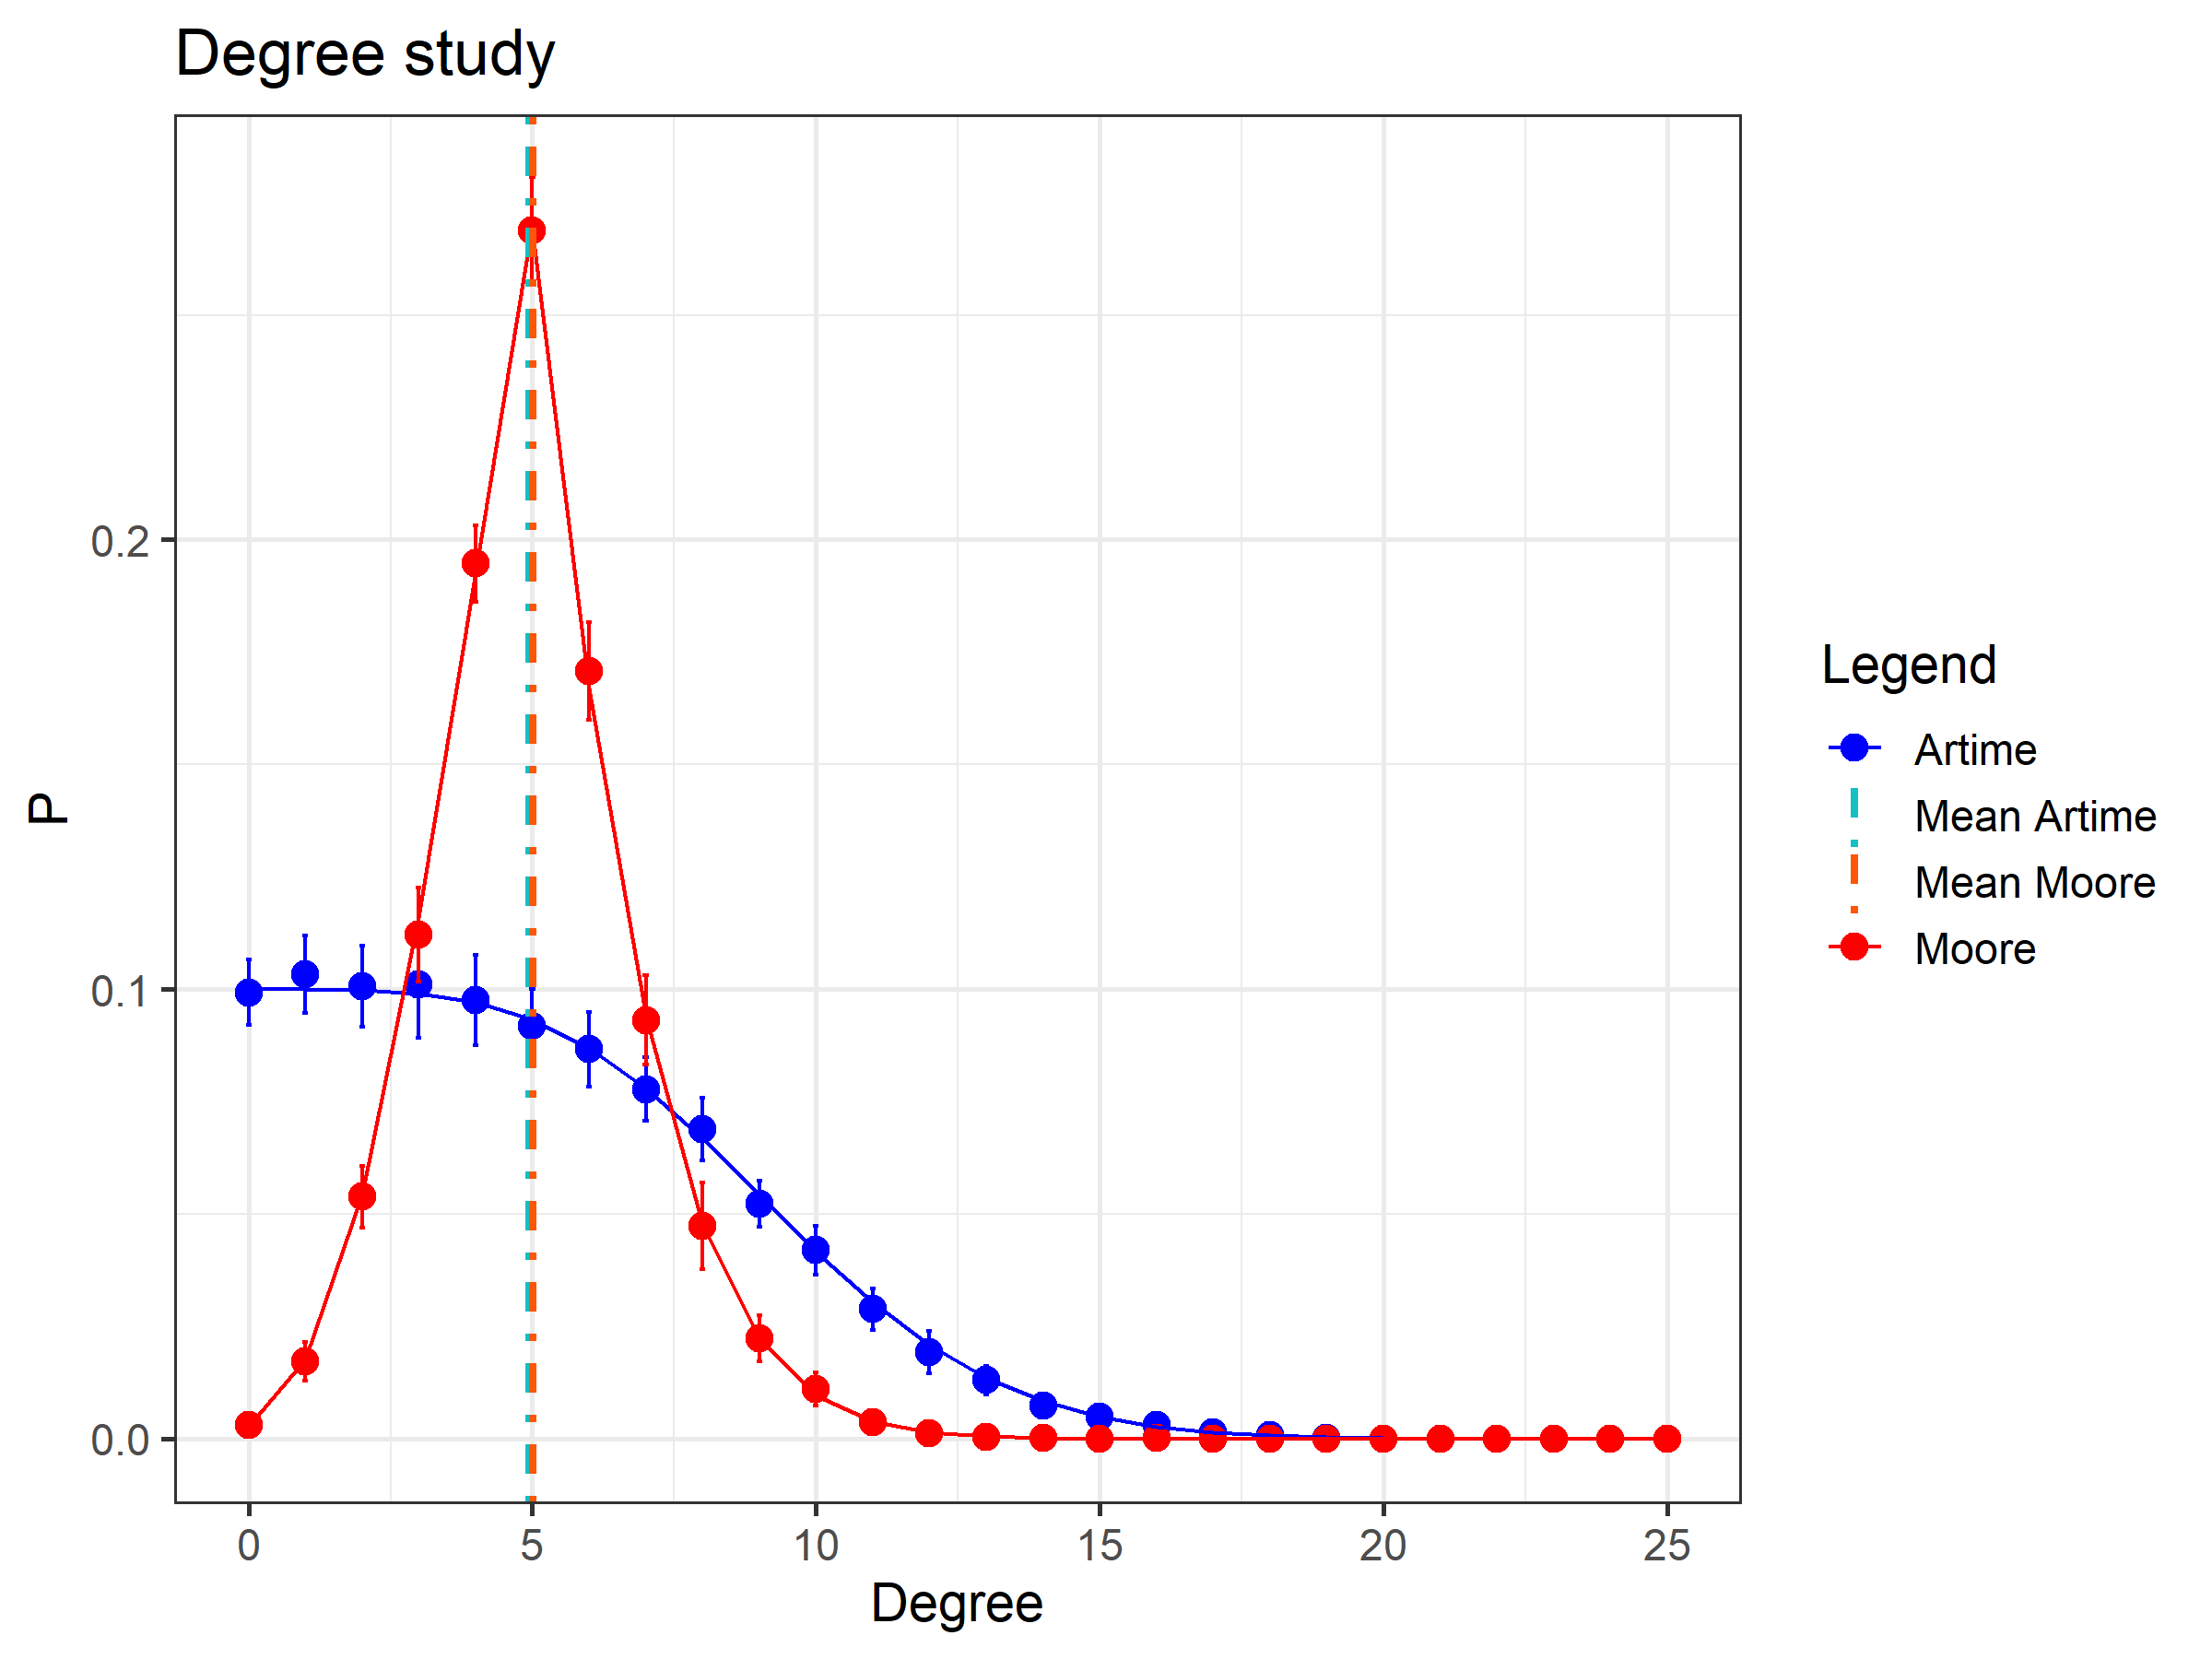
\includegraphics[width=1\textwidth]{images/degree_distribution_20_5000_aprime.png}
    }

    \caption{Network size: 1000; Time-steps: 5000; Iterations: 20}
    \label{fig:deg_dist}
\end{figure}

In figure \ref{fig:deg_dist} we can see the final degree distribution for the two methods. For both of them it was used an initial network with 1000 nodes and no edges. Then the evolution was brought on for 5000 time-steps with values: $\alpha_a = 10/1000$ and $r_a=1/1000$ for Artime's method and $\alpha_m = 5$ and $r_m=1$ for Moore's method.
In this figure we see that, for both models, the data coming from the simulations align with the theoretical prediction from task 1.
Confronting the two models, we can see that both have mean degree tending to 5, as expected. Moore's method, however, has a sharper degree in which, obviously, the maximum probability is associated with 5, the number of new edges given to each reset node. Artime's distribution is instead smoother, with 0 being one of the most likely degree in the network, since the reset nodes are left with no edges.



\section{Size of the LCC}

Secondly we have analysed the appearance of a Largest Connected Component (LCC), looking at its size.


\begin{figure}[h!t]
\centering
    
    \subfigure{
    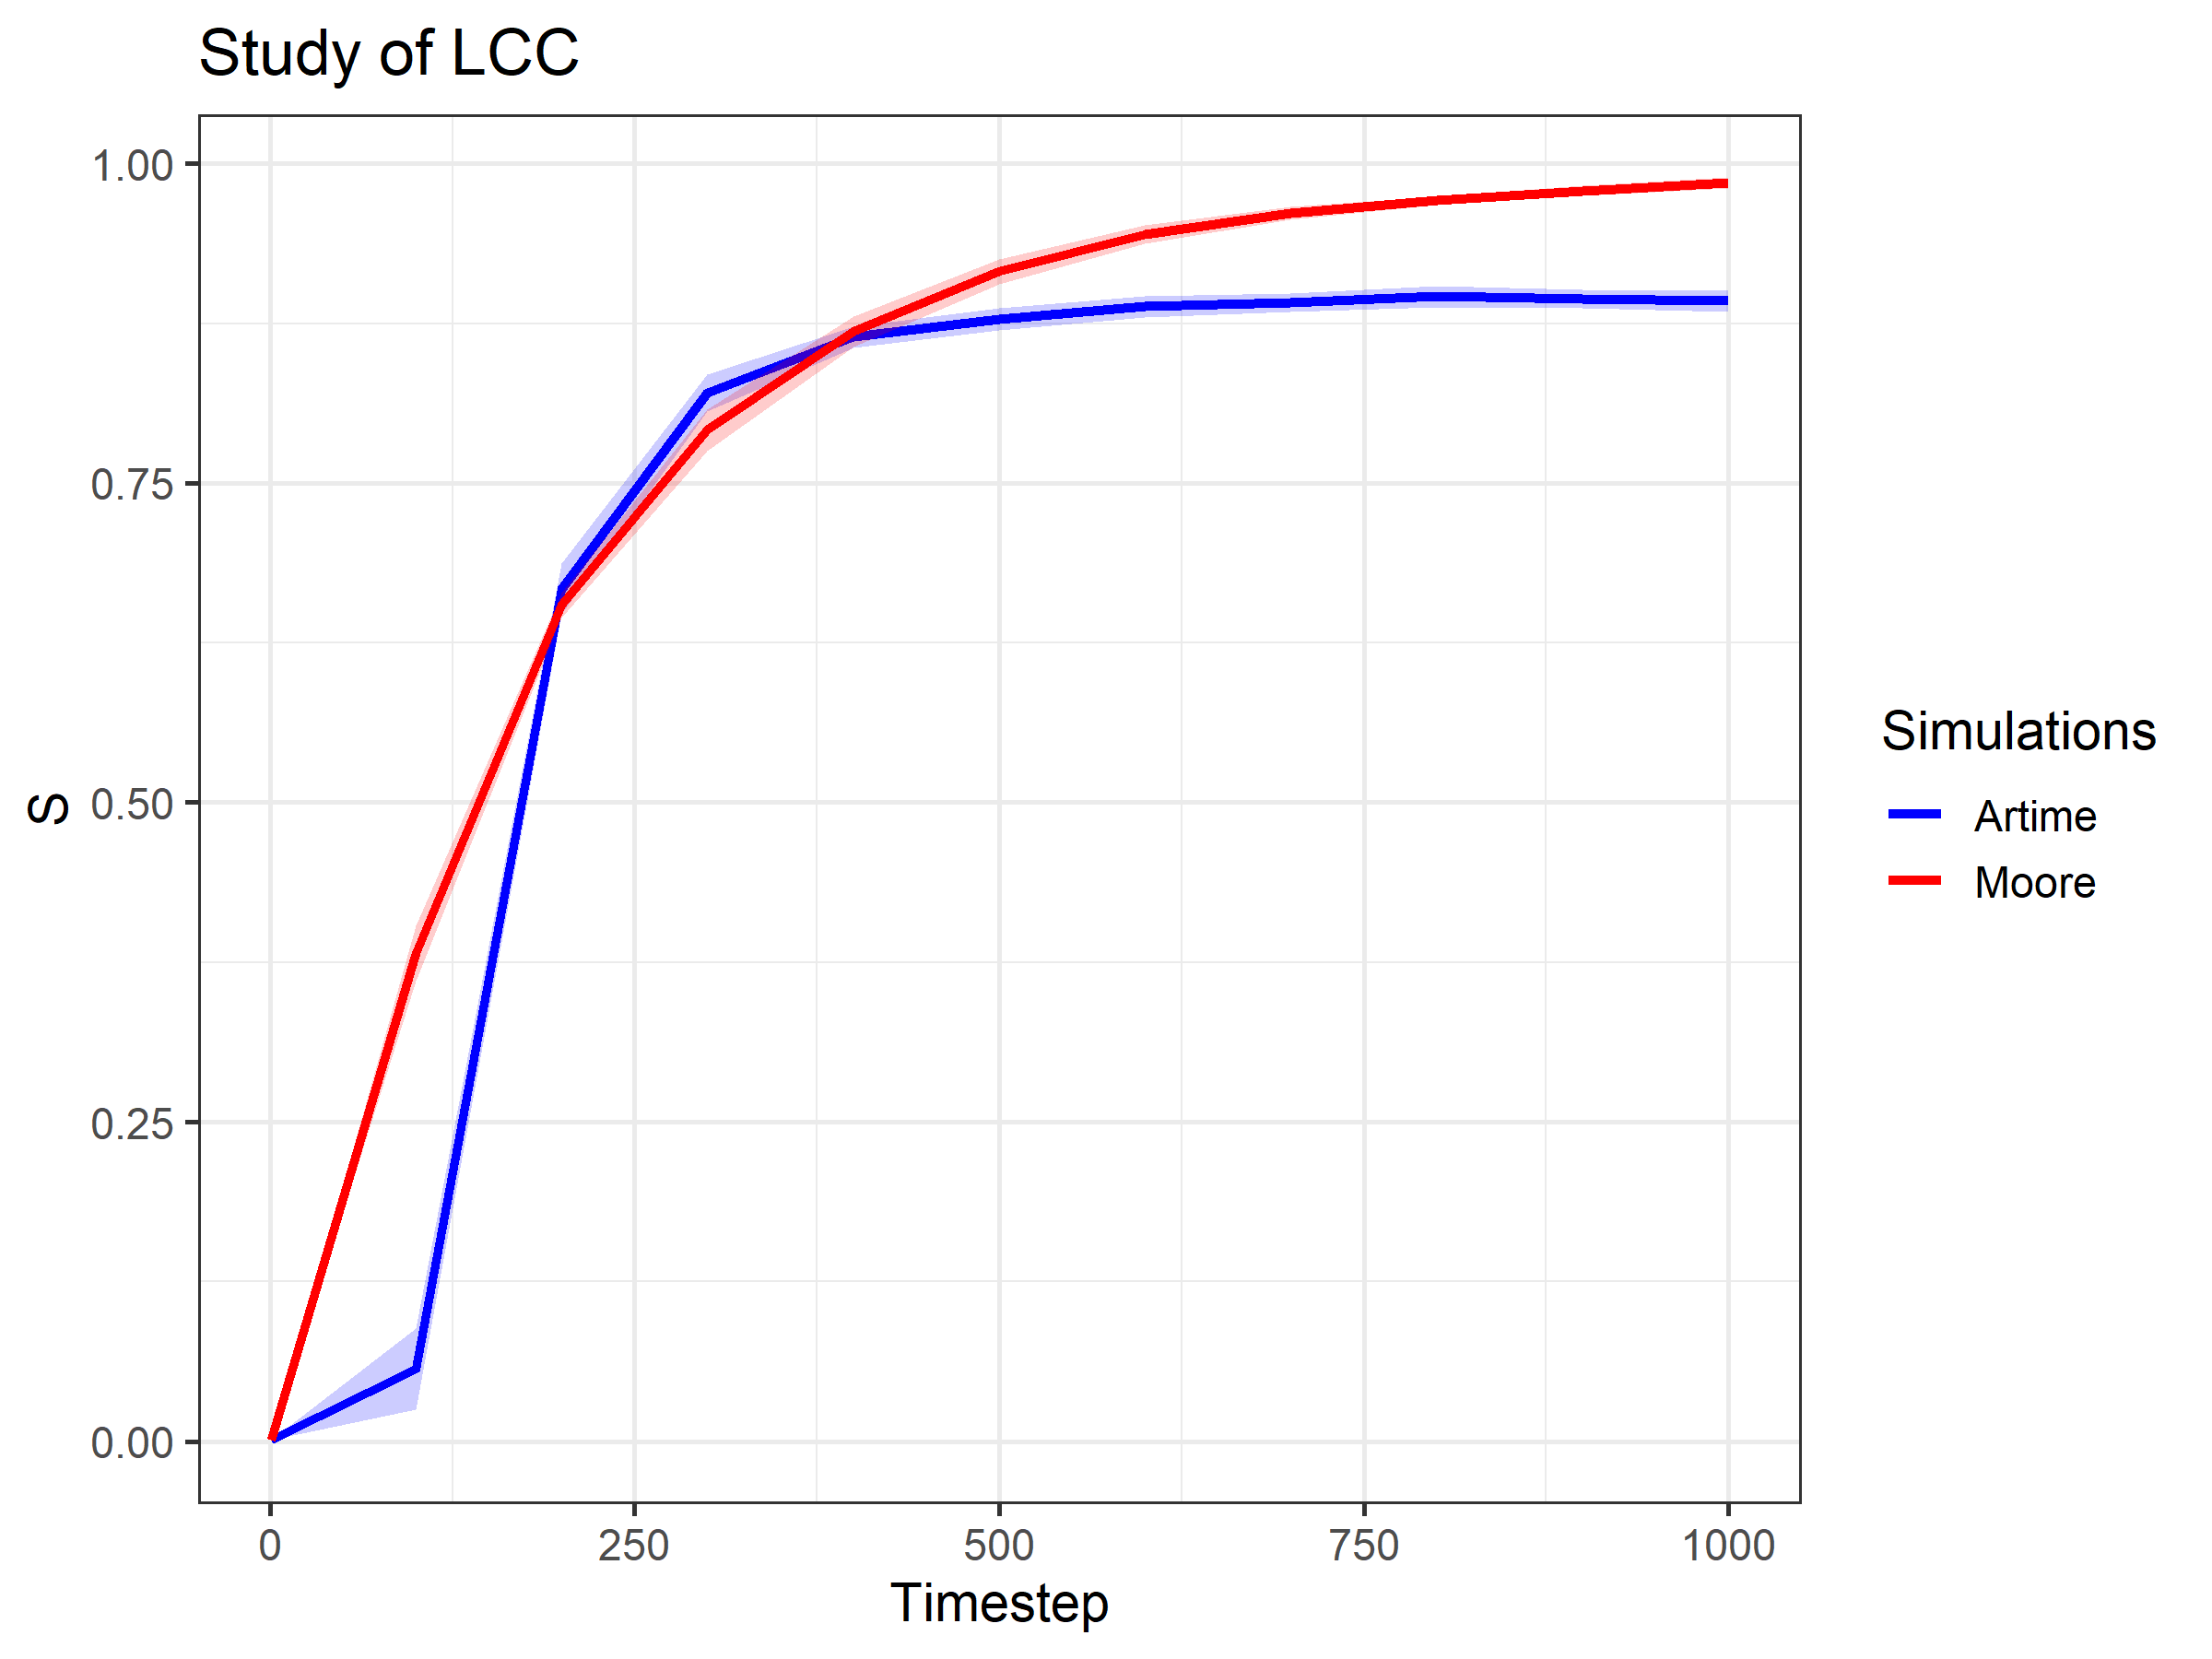
\includegraphics[width=1\textwidth]{images/Size_lcc_20_1000_aprime.png}
    }

    \caption{Network size: 1000; Time-steps: 1000; Iterations: 20}
    \label{fig:lcc}
\end{figure}

In figure \ref{fig:lcc} we report the outcome of a simulation run for 1000 time-steps and with the same initial network and parameters set before. We can see the emergence of an LCC in both models. However, while Moore's network seems to start immediately to form a well connected cluster, Artime's one starts with a flatter curve. We can also notice that, on the contrary, Artime's curve has a sharper transition. Finally, Moore's model builds a more connected network in which almost all node belong to the LCC, although, even for Artime's network we reach a very well connected structure. 

In conclusion, Both models are well described theoretically and show similarity in their final outcome. However, their different approach leads also to significant diversities that could be compared with the real world complex systems, in order to apply to them the more suitable model.

\newpage